\documentclass{article}
\usepackage[german]{babel}
\usepackage{csquotes}
\usepackage[style=apa, backend=biber]{biblatex}
\usepackage[a4paper,top=2cm,bottom=2cm,left=3cm,right=3cm,marginparwidth=1.75cm]{geometry}
\usepackage{fontspec}
\usepackage[colorlinks=true, allcolors=blue]{hyperref}
\usepackage{graphicx}

\setmainfont{Arial}

\addbibresource{references.bib}


\title{
    Transferarbeit
    \\St.Galler Management-Modell
    \\SBB Cargo AG}
\author{
    Jeremy Schuler\\
    Jonas Voland
}

\begin{document}
\begin{titlepage}
    \maketitle
\end{titlepage}

\setcounter{page}{2}

\begin{abstract}
In dieser Arbeit nehmen wir die SBB Cargo AG als Unternehmen in das Zentrum des St. Galler Managment-Modell.
Im ersten Kapitel wird das Unternehmen kurz vorgestellt.
Danach wird das Umfeld in den Bereichen Umweltsphären, Anspruchsgruppen und Wettbewerbssitiation analysiert.
Daraus werden Chancen und Gefahren aufgezeigt und die möglichen Handlungsoptionen.
Abgeschlossen wird mit einer Empfehlung für die SBB Cargo AG.
\end{abstract}

\tableofcontents

\newpage

\section{Das Unternehmen}

Als erstes schauen wir uns die SBB Cargo AG als Unternehmen an.

\begin{figure}[htbp] % h bedeutet "here" und gibt an, dass das Bild hier eingefügt werden soll
    \centering
    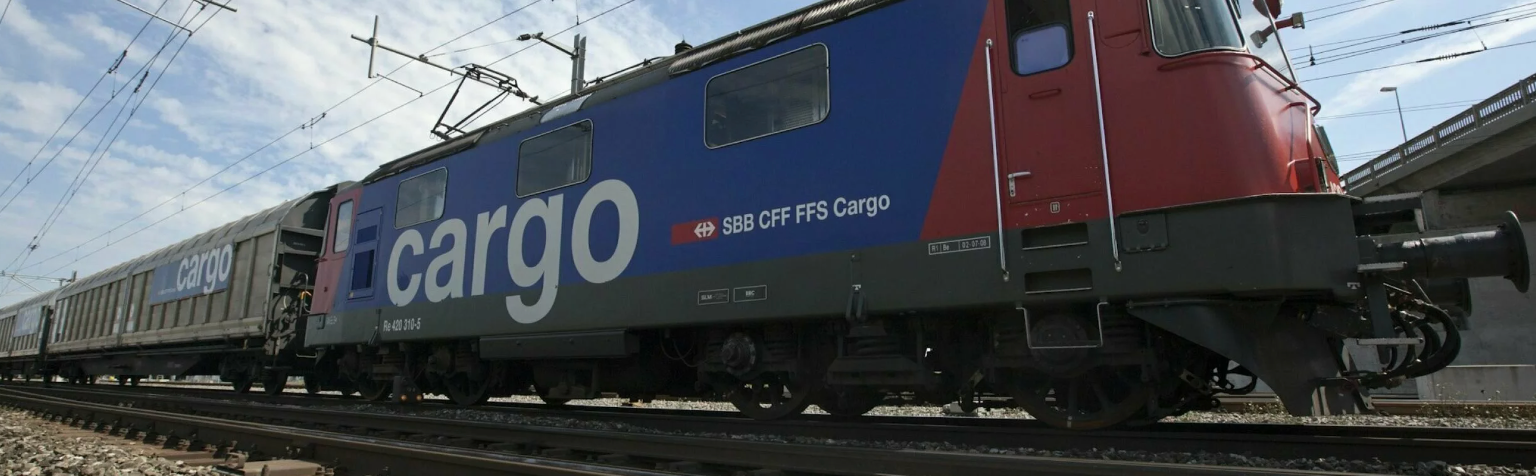
\includegraphics[width=0.75\textwidth]{sbbcargoag} % Ersetze "bilddatei" durch den Dateinamen deines Bildes (ohne Dateiendung)
    \caption{Zug SBB Cargo AG}\parencite[o. S.]{sbbcargoagBild}
    \label{fig:bildlabel2}
\end{figure}

\subsection{Organisation}

Die SBB Cargo AG wurde 1999 gegründet und ist ein Eigenständiges Tochterunternehmen der SBB AG.
Die SBB AG besitzt 100\% der Aktienanteile und ist somit die alleinige Inhaberin der SBB Cargo AG.
Das Top Management besteht aus 8 Personen \parencite[o. S.]{managmentOrganigram}.
% Quelle: https://www.sbbcargo.com/de/unternehmen/organisation/management-organigramm.html
Der Hauptsitz ist in Olten an der Bahnhofstrasse 12 \parencite[o. S.]{standorte}.
% Quelle: https://www.sbbcargo.com/de/unternehmen/organisation/standorte.html
Die SBB Cargo AG hat wiederum auch eine Tochterfirma ChemOil Logistics AG \parencite[o. S.]{chemOil}.
% Quelle: https://www.sbbcargo.com/de/unternehmen/organisation/chemoil-logistics-ag.html

\subsection{Geschäftsbereiche}

Die SBB Cargo AG fokussiert sich auf den Gütertransport in der Schweiz.
Dabei bieten sie zwei Hauptbereiche and und ein Zusatzbereich an.
Einer der zwei Hauptbereiche ist das Transportangebot welches bestehen aus Wagenladungsverkehr, Ganzzüge, Kombinierter Verkehr, Bau \& Baulogistik und Entsorgung \& Recycling besteht.
% TODO: Evtl. ein Diagramm für die Übersicht 
Der zweite Hauptbereich ist das Angebot Rollmaterial, welcher aus den folgenden Teilen besteht. Flottenmanagement \& Service, Instandhaltung SBB Cargo AG und Vermietung von Rollmaterialien. 
Der Bereich Zusatzleistungen wird aufgeteilt in Bahn nahe Logistikleistungen und Services für Bahnunternehmen \parencite[o. S.]{angebot}.
% Quelle: https://www.sbbcargo.com/de/angebot.html

\subsection{Grösse des Unternehmens }

SBB Cargo AG deckt rund ein Siebtel des Schweizer Güterverkehrs ab.
Im Jahr 2021 hatte das Unternehmen einen Umsatz von 777 Millionen.
In Zahlen sind das 5.0 Milliarden Nettotonnenkilometer.
Die oben genannten Leistungen werden Stand 2022 von 2178 Mitarbeitern geleistet.
Die Miterbeiter zahl sinkt über die letzten 5 Jahren leicht \parencite[o. S.]{personal}.
% Quelle: https://reporting.sbb.ch/personal?highlighted=f8ce472b9748ab288816aa3fc328a6d2&years=1,4,5,6,7&scroll=480
Die Wirtschaftliche Lage ist brisant.
Laut dem Geschäftsbericht 2022 fährt die SBB Cargo AG einen Verlust von 187.4 Millionen CHF ein.
Im Jahr 2021 schaffte das Unternehmen noch einen Gewinn von 1.1 Millionen \parencite[S. 46]{geschaeftsbericht2022}.
% Quelle: https://www.sbbcargo.com/de/medien/publikationen/geschaeftsberichte.html

\subsection{Kunden/Zielgruppen}

Die Zielgruppe von SBB Cargo AG sind in erster Linie Unternehmen, die Bedarf an Gütertransport haben.
Zu den Zielgruppen gehören auch Firmen, welche Bedarf an Langstrecken Transport haben und da bei auf eine Ökologische und zuverlässige Lösung angewiesen sind.
Die Kunden von der SBB Cargo AG kommen zum grössten Teil aus der Industrie, Produktion oder Logistik.

\subsection{Konkurrenten}
Folgende 9 Unternehmen zählen zu den grössten Gütertransportunternehmen in der Schweiz nach Umsatz im Jahr 2021 und stehen somit in Konkurrenz:
\begin{itemize}
\item Lagerhäuser der Centralschweiz AG (1.84 Millionen CHF)
\item Bertschi AG (1.03 Millionen CHF)
\item Planzer Holding AG (986 Millionen CHF)
\item Galliker Transport AG (700 Millionen CHF)
\item Hupac SA (682 Millionen CHF)
\item Cargo24 AG (539 Millionen CHF)
\item Rhenus Alpina AG (476 Millionen CHF)
\item Schenker Schweiz AG (305 Millionen CHF)
\item Loomis Schweiz AG (280 Millionen CHF)
\end{itemize}
\parencite[o. S.]{groessteUnternehmenGuetertransport}
% Quelle: https://de.statista.com/statistik/daten/studie/1050561/umfrage/groesste-schweizer-guetertransportunternehmen-nach-umsatz/

\subsection{Partner / Lieferanten}
Der Strom, für den Antrieb der Züge, wird von der SBB AG grösstenteils produziert.
Ergänzend wird der Bedarf durch Beteiligungen und Bezugsverträge gesichert \parencite[o. S.]{verbrauch}.
% Quelle: https://company.sbb.ch/de/sbb-als-geschaeftspartner/leistungen-evu/energie/verbrauch.html
Ein wichtiger strategischer Partner ist die Swiss Combi AG. 
An dem Unternehmen sind die Logistikdienstleister Planzer Holding AG (40\%), Camion Transport AG (40\%), Bertschi AG (10\%) und Galliker Holding AG (10\%) beteiligt.
Zusammen wollen sie den Wagenladungsverkehr und die Verlagerungspolitik aktiv vorantreiben \parencite[o. S.]{sbbGueterZukunft}.
% Quelle: https://news.sbb.ch/medien/artikel/123195/sbb-stellt-sich-fuer-den-gueterverkehr-der-zukunft-auf
Und PJ Messtechnik GmbH bietet System Lösungen für den Schienenverkehr an, welche die SBB Cargo AG einsetzt \parencite[o. S.]{partnerPJMesstechnik}.
% Quelle: https://blog.sbbcargo.com/sbb-cargo-die-rail-cargo-group-und-pj-messtechnik-arbeiten-am-intelligenten-gueterzug/

\section{Analyse des Unternehmensumfeldes}

Nun analysieren wird das Umfeld der SBB Cargo AG.

\subsection{Umweltsphären}

Hier schauen wir die verschiedenen Umweltspähren des St. Galler Managment-Modell an.

\subsubsection{Ökologische Umweltsphäre (Natur)}

\begin{itemize}
\item Umweltschutz:
Die SBB Cargo AG ist grundsätzlich was die Ökologischen Aspekte der heutigen Zeit angeht nicht im Nachtreffen wie andere Firmen.
Dies ist darauf zurückzuführen das das ganze Güternetz, welches betrieben wird, eine CO2 Ersparnis von 490 000 Tonnen pro Jahr einbringt.
% TODO: Quelle: FEHLT

\item Umweltverschmutzung:
Eine der Grössten Klima Belastungen sind die Fahrten von Diesellokomotiven auf strecken, welche nicht elektrifiziert sind.   

\item Energieverbrauch: Im Bereich des Schienenverkehrs ist die Energie auch immer ein grosses Thema da es darum geht den Strom von möglichst nachhaltigen Quellen zu beziehen, ansonsten hat man nicht die gewünschte Umweltfreundlichkeit. 
Die SBB AG sagt das sie aktuell mit 90\% Energie aus Wasserkraft fährt und 10\% Energie aus Atomstrom sind. Das Ziel der SBB AG ist die 10\% Atomstrom mit Strom aus eigenen Anlagen oder aus Anlagen, welche unter Vertrag stehen zu ersetzen.
\item Gotthard Basistunnel:
Der Umfall im Gotthard Basistunnel führte dazu, dass für eine länger Zeit die Strecke nicht befahren werden konnte.
Die Umleitung über die Panoramastrecke darf von Güterzügen nur sehr beschränkt eingesetzt werden.
Das wiederum führte dazu, dass viele Kunden zum Strassentransport gewechselt sind.
\end{itemize}

\begin{figure}[htbp] % h bedeutet "here" und gibt an, dass das Bild hier eingefügt werden soll
    \centering
    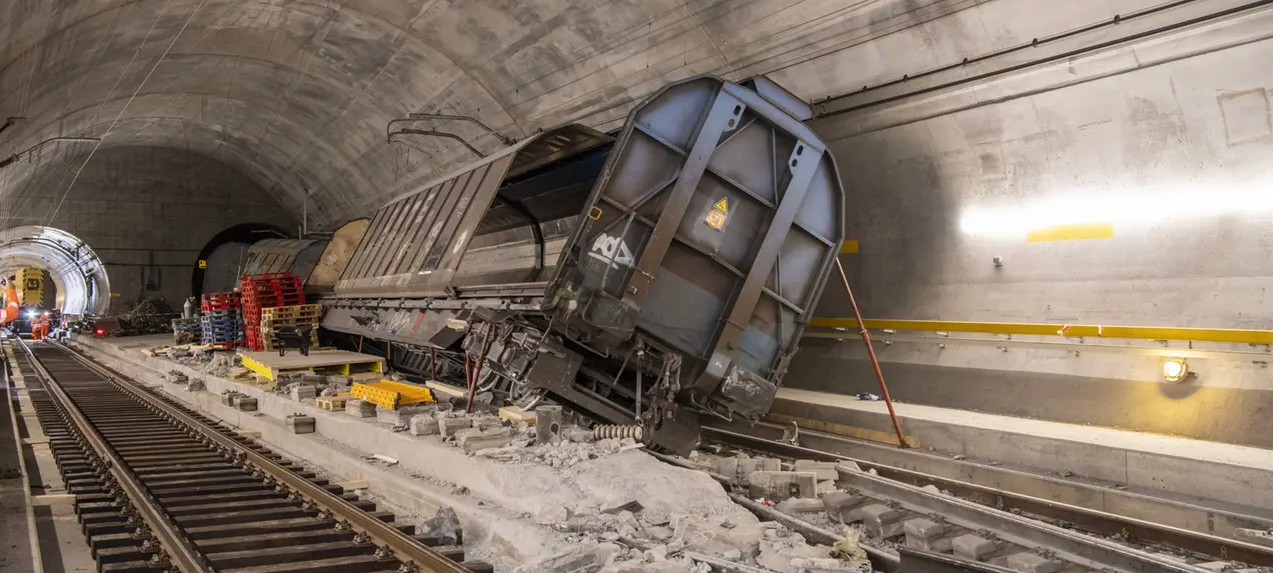
\includegraphics[width=0.75\textwidth]{umfallGotthard} % Ersetze "bilddatei" durch den Dateinamen deines Bildes (ohne Dateiendung)
    \caption{Gotthardtunnel Umfall}\parencite[o. S.]{gotthardtunnelBild}
    \label{fig:bildlabel}
\end{figure}

\subsubsection{Gesellschaftliche Umweltsphäre}

Kulturelle und Soziale Entwicklungen:
\begin{itemize}
\item Lärm: Der Lärm ist in der Bevölkerung ein grosses Thema. Direkte Anwohner bei Schienennetzen fordern einen Lärmschutz. 
\end{itemize}
Politische und rechtliche Entwicklungen:
\begin{itemize}
\item Lärm: Politisch wurde auch auf das Thema Lärm reagiert und seit 2020 dürfen nur noch lärmsanierte Güterwagen in der Schweiz verkehren.
\end{itemize}
\parencite[o. S.]{umwelt}
% Quelle: https://www.sbbcargo.com/de/unternehmen/qualitaet-sicherheit-umwelt/umwelt.html 

\subsubsection{Technologische Umweltsphäre}

Die SBB Cargo AG innoviert durchgehend und setzt auf neue Technologien.
\begin{itemize}
    \item Automatische Kupplung: Seit 2019 sind Loks mit automatischen Kupplungen im Betrieb.
    \item Automatische Bremsprobe: Die Technologie wird vom Partner PJ Messtechnik eingekauft und damit können in nur 10 Minuten automatische Bremsproben durchgeführt werden.
    \item Kollisionswarnsystem: Es werden Kollisionswarnsystem eingesetzt. Der Arbeiter wird beim Rangieren durch visuelle und akustische Signale vor Hindernissen gewarnt.
    \item Cargo Check-In: Diese ist eine mobile App, welche dem Kunden ermöglich selbst den Check-in-Prozess an der Rampe via Smartphone vorzunehmen.
    \item Cargo View: Durch die neue Web-Applikation “Cargo View” bekommt der Kunde eine Übersicht zu all seinen Sendungen.
    \item Mobile Wagenkontrolle: Mit einer neuen App zur mobilen Wagenkontrolle wird ermöglicht die Wagen ein zu Checken Schäden an der Fracht festzuhalten und alles zu überwachen.
    \item Predictive Maintanance: Mit Hilfe von Sensoren und Kameras werden Daten gesammelt, welche in Zukunft dazu dienen wird, eine effizientere Wagen Wartung zu betreiben.
    \item Wayside Kamera: Mit Hilfe von Kameras werden Schäden an Fahrzeugen detektiert und diese direkt an die Zuständigen Personen weitergeleitet. Dies dient zur Steigerung der Sicherheit im Verkehr.
\end{itemize}
\parencite[o. S.]{innovation}
% Quelle: https://sbbcargo.pageflow.io/innovation - 127546 


\subsubsection{Ökonomische Umweltsphäre (Wirtschaft)}
Gesamtwirtschaftliche Einflüsse:
\begin{itemize}
    \item Verlagerungspolitik:
    Wirtschaftspolitisch wird in der Schweiz die Verlagerungspolitik geführt.
    Dadurch sollen politische Massnahmen definiert werden, die den Güterverkehr nachhaltig von den Strassen auf die Schienen gebracht werden, soll \parencite[o. S.]{verlagerungspolitik}.
    % Quelle:  https://blog.sbbcargo.com/der-schienengueterverkehr-ist-zentral-fuer-eine-funktionierende-wirtschaft/
    Ein aktuelles Beispiel wäre das Gateway Basel Nord.
    Dort wurde vom Bundesamt für Verkehr (BAV) die Plangenehmigungsverfügung erteilt \parencite[o. S.]{gatewayBasel}.
     % Quelle: https://www.wsu.bs.ch/nm/2023-die-plangenehmigung-fuer-das-gateway-basel-nord-staerkt-den-logistikstandort-basel-und-die-verlagerungspolitik-des-bundes-wsu.html 
    Damit sollen mehr Güter vom Strassenverkehr auf die Schienen kommen.
\end{itemize}
\begin{figure}[htbp] % h bedeutet "here" und gibt an, dass das Bild hier eingefügt werden soll
    \centering
    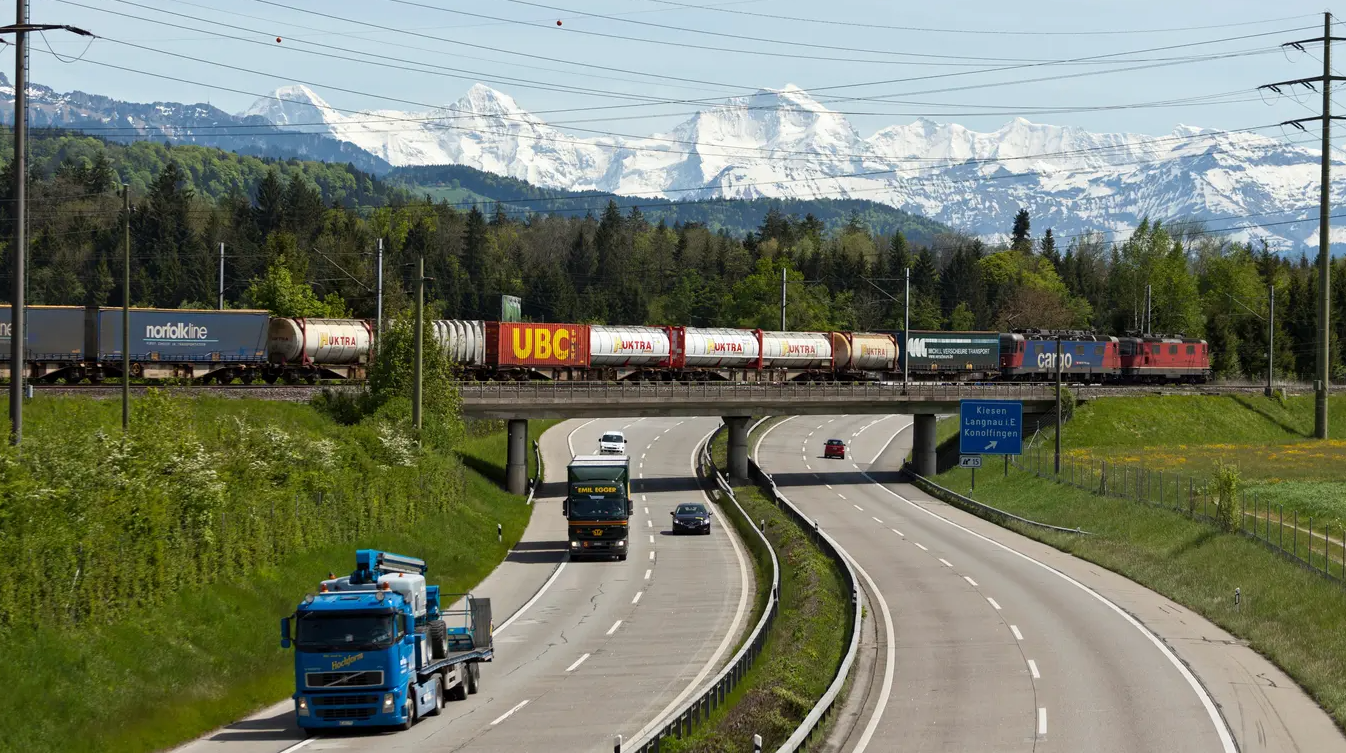
\includegraphics[width=0.75\textwidth]{Verlagerungspolitik} % Ersetze "bilddatei" durch den Dateinamen deines Bildes (ohne Dateiendung)
    \caption{Symbolisch Verlagerunspolitik}\parencite[o. S.]{verlagerungspolitikBild}
    \label{fig:bildlabel3}
\end{figure}
Markt und Konkurrenz:
\begin{itemize}
    \item Globalisierung:
    Durch die Globalisierung nimmt der Bedarf für den Transport von Gütern stetig zu.
    Die bringt neue Kunden, jedoch bringt das auch neue Konkurrenten aus dem Ausland. 
\end{itemize}

\subsection{Anspruchsgruppen}

Jetzt kommen die Anspruchsgruppen des St. Galler Managment-Modell.

\subsubsection{Kapitalgeber}
Die Finanzierung von der SBB Cargo AG ist durch die SBB AG sichergestellt, welche von dem Bund finanziert wird.
Jedoch durch die hohen Verluste wird die SBB Cargo AG den Ansprüchen, dass sie eine sichere und wertseigernde Kapitalanalage ist, nicht gerecht.
Forderung ist, dass der Gütertransport optimiert wird, um Gewinne zu ermöglichen.

\subsubsection{Kunden}
Durch die Globalisierung fordern Kunden, dass Güter immer effizienter, schneller und in grösseren Mengen transportiert werden können.
Sie wollen auch, dass die Waren unbeschädigt ankommt.

\subsubsection{Mitarbeitende}
Die Lokführer wollen mit modernen Zügen arbeiten können, da diese mehr Sicherheit und Komfort bieten.
Es hat auch den Effekt, dass es spannender ist mit modernen Zügen zu arbeiten. 

\subsubsection{Öffentlichkeit}
Durch die Grösse und Nähe zum Bund verfolgen die Medien das Unternehmen sehr stark und fordern Transparenz.

\subsubsection{Staat}
Der Staat gibt die Rahmenbedingung vor und hat die Erwartungen, dass diese auch eingehalten und überwacht werden.
Er fordert auch vom Unternehmen finanzielle Beiträge für die Bewältigung öffentlicher Aufgaben durch Steuern und Abgaben.
Durch die indirekte Beteiligung an der SBB Cargo AG, hat der Bund ein starkes Eigeninteresse die Verlagerungspolitik nach vorne zu bringen.
Forderung ist, dass die SBB Cargo AG Gütertransport über die Schienen ermöglicht.

\subsubsection{Lieferanten}
Durch die kritische Finanzielle Lage könnten die Lieferanten Bedenken haben, dass die SBB Cargo AG die Rechnungen bezahlen können.
Das könnte dazu führen, dass sie nur per Vorauszahlung liefern.

\subsubsection{Konkurrenz}
Die Konkurenz möchte, dass die Infrastruktur, welche für den Transport benötigt wird, fair aufgeteilt und benutzt wird.


\subsection{Wettbewerbssituation}
Die Wettbewerbssituation von SBB Cargo AG kann sich je nach Region, Art der Transportdienstleistungen und anderen Faktoren unterscheiden.
Folgende Aspekte können die Wettbewerbssituation beeinflussen könnten: 

\begin{itemize}
    \item Andere Bahngesellschaften:
    In der Schweiz gibt es neben der SBB Cargo AG auch andere Bahngesellschaften, die im Güterverkehr tätig sind.
    Wettbewerber könnten inländische oder ausländische Unternehmen sein, die ähnliche Dienstleistungen anbieten. 
    \item Straßentransportunternehmen:
    SBB Cargo AG konkurriert auch mit Unternehmen im Straßentransportsektor, da Straßenfracht eine alternative Transportmöglichkeit für Güter darstellt. 
    \item Logistikunternehmen:
    Logistikunternehmen, die verschiedene Transportmodalitäten anbieten, könnten ebenfalls als Wettbewerber agieren, wenn sie Güterverkehrsleistungen auf der Schiene erbringen.
    \item Marktentwicklungen:
    Veränderungen in der Nachfrage nach Güterverkehrsleistungen, technologische Entwicklungen und regulatorische Veränderungen können die Wettbewerbssituation beeinflussen. 
\end{itemize}

\section{Ermittlung von Chancen und Gefahren für SBB Cargo AG}

Bezogen auf die Analyse des Umfeldes möchten wir Chancen und Gefahren aufzeigen.

\subsection{Chancen}
\begin{itemize}
    \item Das Basel Bauprojekt
    \item Die viele neuen Technologischen Entwicklungen.
    \item Die Verlagerungspolitik.
    \item Globalisierung des Gütertransportes
\end{itemize}
\subsection{Gefahren}
\begin{itemize}
    \item Die Kunden, die wegen dem Umfall im Gotthardtunnel auf den Strassenverkehr gewechselt sind, kommen nicht mehr zurück.
    \item Die hohen Verluste führen zu grosser Unsicherheit bei den Kapitalgebern und Lieferanten.
    \item Verlust von Kunden an ausländische Transportunternehmen.
\end{itemize}

\section{Handlungsoptionen}

Folgende Handlungsoptionen stehen der SBB Cargo AG offen:

\begin{itemize}
    \item Abschluss des Basel Bauprojektes nutzen da man dadurch in der Region einen grösseren Transportbedarf abdecken kann. 
    \item Neue Technologien einsetzen, um betrieb zu optimieren und so Kosten einzusparen und die grossen Verluste zu verkleinern. 
    \item Den Transport optimieren, damit sie einen günstigeren Transport anbieten können. 
    \item Sich verstärkt einsetzen für Verlagerungspolitik, um so neue Kunden zu gewinnen und ausländische Unternehmen auszustechen. 
    \item Die Globalisierung nutzen um sich verstärkt im Ausland auszubreiten. 
\end{itemize}

\subsection{Vorteile Handlungsoptionen}
\begin{itemize}
    \item Vergrösserung des Unternehmens um damit neue und verbesserte Erschliessung der Region sicherzustellen. 
    \item Einsparung von Kosten für Unterhalt sowie verbesserte Arbeitsbedingungen für angestellte. 
    \item Durch das Senken der Kosten könnte man das schlechte Geschäftsjahr ausbessern. 
    \item Es besteht eine gute Möglichkeit mehr Kunden für den Schienen Transport zu gewinnen da man den Gütertransport in diese Richtung drängt. 
    \item Erweiterung des Internationalen Einflusses. 
\end{itemize}

\subsection{Nachteile Handlungsoptionen}
\begin{itemize}
    \item Ein Hoher Finanzieller aufwand.
    \item Man muss in die Technologien investieren, um danach erst Kosten zu sparen. 
    \item Man muss eine konkrete Herangehensweise haben, ansonsten wird es nicht rentabel für die SBB Cargo AG 
    \item Man muss attraktives Angebot bereit stellen um die wechselnden Kunden nicht an anderen Transport unternehmen zu verlieren 
\end{itemize}

\section{Empfehlungen für SBB Cargo AG}

Eine Empfehlung ist bestimmt das man den Fokus auf das Projekt in Basel legt, das man mögliche Neukunden nicht verpasst welche in diesem Fall recht einfach zu Gewinnen währen.
Dazu kommt, dass sie möglichst die Kosten günstigsten Chancen, nutzen sollten da sie im letzten Jahr finanziell eher nicht optimal gewirtschaftet haben.
Sie sollten im aktuellen Zustand möglichst mit kleinem Kosten aufwand sich vergrössern und optimieren, um in Zukunft mehr Gewinn zu erzielen und Kosten günstiger zu Transportieren. 

\section{Eigenständigkeitserklärung}

Hiermit erklären wir, dass wir diese Arbeit ohne fremde Hilfe und ohne Verwendung anderer als angegebener Hilfsmittel verfasst haben.

\begin{center}
\begin{tabular}{ c c }
    Jeremy Schuler & Jonas Voland\\
\end{tabular}
\end{center}
Bern, \today

\cleardoublepage
\printbibliography[title={Literaturverzeichnis}]
\addcontentsline{toc}{section}{Literaturverzeichnis}

\newcommand{\listoffiguresintoc}{
    \cleardoublepage
    \phantomsection
    \addcontentsline{toc}{section}{\listfigurename}
    \listoffigures
}
\listoffiguresintoc


\end{document}